\chapter{Conjuntos numéricos}

 \section{Conjunto dos números Naturais (\texorpdfstring{$\N$}{N})}

Os registros mais antigos de números encontrados na história, são de símbolos que eram utilizados para registrar a quantidade de animais, estes símbolos foram sendo aprimorados com o desenvolvimento das sociedades e o aprimoramento da escrita, chegando ao sistema de numeração hindu-arábico que são os números como conhecemos hoje.

Este números que ainda utilizamos para a contagem de objetos são denominados números naturais, como por exemplo:
\[\N= \{0, 1, 2, 3, 4, 5, \cdots \},\]
e o conjunto dos números naturais sem o zero.
\[\N^{*}= \{1, 2, 3, 4, 5, \cdots \}.\]

O zero foi o último deles a ser criado, já que no início não havia necessidade de registro no caso de não se ter posses.
Ainda se discute dentro da matemática se o zero pertence ou não ao conjunto dos números naturais.

É importante notar que neste conjunto numérico temos bem definida apenas a operação de soma/adição (+).

\section{Conjunto dos números Inteiros (\texorpdfstring{$\Z$}{Z})}

Com o surgimento do comércio, surge a necessidade dos comerciantes de registrarem a entrada e saída de bens em seus estabelecimentos, bem como seus lucros e suas despesas. Para efetuar estes registros eles criaram os números negativos, tendo assim como registrar posses usando números positivos e dívidas usando os números negativos.

Este conjunto de números negativos juntamente com os números naturais, forma o conjunto dos números inteiros:
\[\Z= \{ \cdots, -5, -4, -3, -2, -1, 0, 1, 2, 3, 4, 5, \cdots \}\]

Observe que $\N \subset \Z$. E ainda que no conjunto dos números inteiros temos bem definidas as operações de soma (+) e subtração (-).

\section{Conjunto dos números Racionais (\texorpdfstring{$\Q$}{Q})}

Note que no conjunto dos números inteiros ainda não é possível fazer todas as divisões, por exemplo $3 \div 2$ ainda não está definida, pois ainda não existe um número que represente este resultado. Para resolver este problema surge então o conjunto dos números racionais, que é formado por todos os números que podem ser escrito em forma de fração, ou seja o conjunto dos números que podem ser obtidos como resultado de alguma divisão, representamos este conjunto por:
\[\Q= \{ \left(\frac{a}{b}\right); a, b \in \Z \text{ e } b \neq 0 \}.\]

Observe que $\N \subset \Z \subset \Q$. E ainda que no conjunto dos números racionais temos bem definidas as operações de soma (+), subtração (-), multiplicação/vezes (.) e divisão/razão ($\div$). Porém as operações neste conjunto possuem algumas particularidades com as quais devemos ficar atentos, por isso iremos retomá-las na sequência de nossos estudos.

 \vskip0.3cm
 \colorbox{azul}{
 \begin{minipage}{14.5cm}
 \begin{center}
  Chamamos de \textbf{dízimas periódicas} os números decimais com infinitas casas decimais, nos quais a partir de alguma casa decimal, um algarismo ou um grupo de algarismos passa a se repetir infinitamente. O algarismo ou algarismos que se repetem infinitamente constituem o período da dízima.
 \end{center}
 \end{minipage}}
 \vskip0.3cm

 \begin{exem} Vejamos alguns exemplos de dízimas periódicas, e como dada a dízima encontrar a fração que a representa.

  \begin{enumerate}[a)]
   \item Considere o número $0,333 \cdots$, neste caso o período é $3$, assim,
   \[0,3333 \cdots= 0,\overline{3}= \frac{3}{9}= \frac{1}{3}\]
   De fato,
   \begin{eqnarray*}
    x &=& 0,3333 \cdots \\
    10x &=& 10 \cdot 0,3333 \cdots \\
    10x &=& 3,3333 \cdots \\
    10x &=& 3 + 0,3333 \cdots \\
    10x &=& 3 + x \\
    10x - x &=& 3 \\
    9x &=& 3 \\
    x &=& \frac{3}{9} \\
    0,3333 \cdots &=& \frac{1}{3}
   \end{eqnarray*}
   usando a mesma ideia conseguimos mostrar os exemplos abaixo.

   \item Considere o número $0,121212 \cdots$, neste caso o período é $12$, assim,
   \[0,121212 \cdots= 0,\overline{12}= \frac{12}{99}= \frac{4}{33}\]
   \item Considere o número $0,225225225 \cdots$, neste caso o período é $225$, assim,
   \[0,225225225 \cdots= 0,\overline{225}= \frac{225}{999}= \frac{75}{333}=\frac{25}{111}\]
   \item Considere o número $7,464646 \cdots$, neste caso o número tem uma parte inteira que é $7$ e uma parte decimal $0,464646 \cdots$ na qual o período é $46$. Portanto,
   \begin{eqnarray*}
    7,464646 \cdots &=& 7+0,464646 \cdots \\
    &=& 7 + \frac{46}{99} \\
    &=& \frac{7\cdot 99 + 46}{99}\\
    &=& \frac{739}{99}
   \end{eqnarray*}

  \end{enumerate}

 \end{exem}

Concluímos dos exemplos acima que toda dízima periódica é um número racional, assim como os números inteiros, já que, se $a \in \Z$ então $a=\frac{a}{1}$, portanto $a \in \Q$, e os números com um número finito de casas decimais, por exemplo, $0,15= \frac{15}{100}$.


\section{Conjunto dos números Irracionais (\texorpdfstring{$\I$}{I})}

Com o aprimoramento do cálculo de áreas, vem também a necessidade de sabendo a área, por exemplo do quadrado, descobrir quais as medidas de seus lados, dando então origem ao cálculo das raízes quadradas, surge portanto um novo problema, com os números criados até então nem todo número tem uma raiz quadrada. Para resolver este impasse, criou-se o conjunto dos números irracionais, números estes que não podem ser representados por uma fração como por exemplo: $\sqrt{2}$, $\sqrt{3}$, $\sqrt{5}$, $\sqrt{7}$, pi ($\pi$), número de Euler ($e$), e muitos outros. Observe que $\Q \cap \I = \emptyset$.

Números decimais com infinitas casas decimais que não sejam dízimas periódicas são portanto exemplos de números irracionais.

\section{Conjunto dos números Reais (\texorpdfstring{$\R$}{R})}

O mais fácil de definir de todos os conjuntos numéricos apresentados até então é o conjunto dos números reais, onde todas as 4 operações básicas estão bem definidas. O conjunto dos números reais nada mais é do que a união dos números racionais com os números irracionais, $\R= \Q \cup \I$.

Porém como o produto de dois números negativos, é sempre positivo, neste conjunto não podemos calcular a raiz quadrada de qualquer número real, temos portanto mais um problema a ser resolvido, e para tal os matemáticos criaram então mais um conjunto numérico o conjunto dos números complexos!


\section{Conjunto dos números Complexos (\texorpdfstring{$\C$}{C})}

Para resolver o problema da raiz quadrada de um número negativo, criou-se o número imaginário puro $i$, definido por $i= \sqrt{-1}$, portanto $i^2= -1$, criou-se assim um número $i$ que elevado ao quadrado desse $-1$. Temos agora como calcular a raiz quadrada de qualquer número real. Definimos a partir deste número imaginário o conjunto dos números complexos por:
\[\C= \{a + bi; a, b \in \R \} ,\]
cujas operações apresentam algumas particularidades e portanto trataremos delas mais adiante.

Note que, se tivermos $b=0$, estamos com o conjunto dos números reais, portanto $\R \subset \C$. Para fixar a ordem de continência destes conjuntos numéricos, observemos o diagrama de Venn abaixo.

 \begin{figure}[H]
 \centering
    \fbox{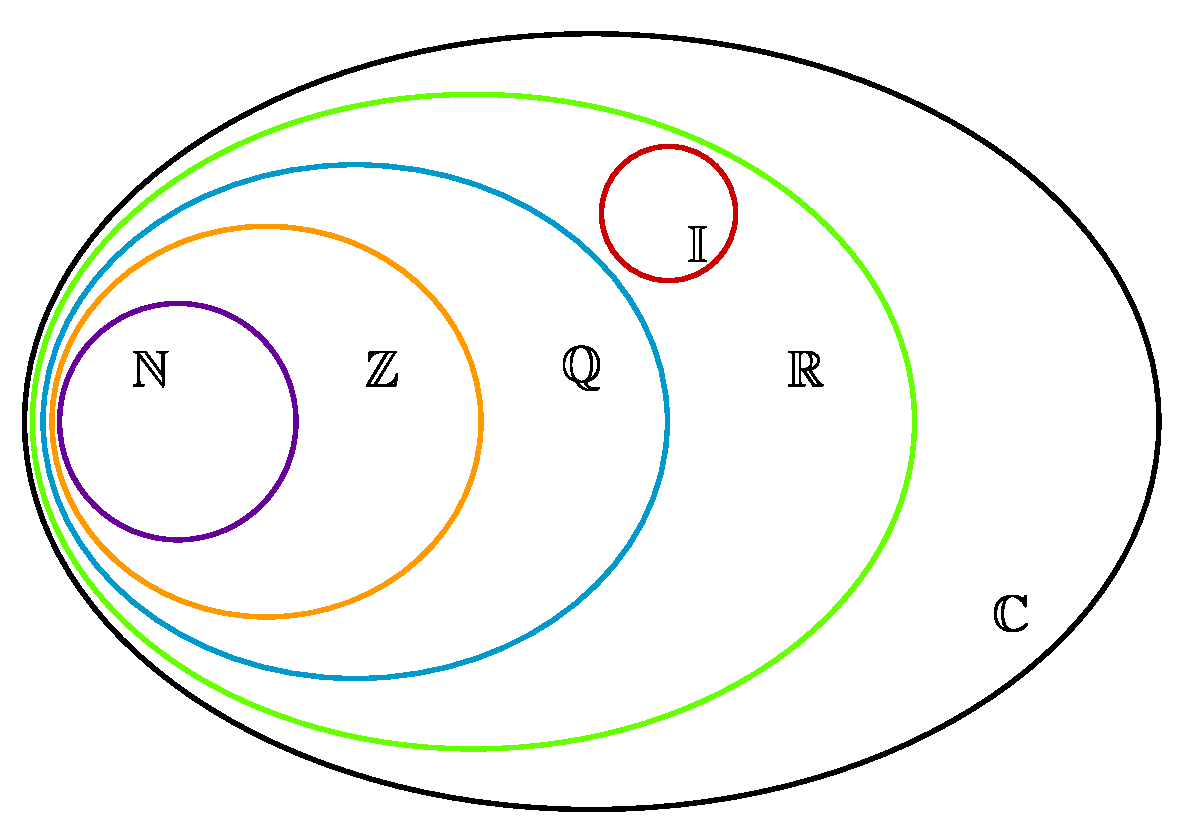
\includegraphics[width=7.5cm]{../Topicos/Figuras/diagrama_conjuntos.pdf}}
    \caption{Representação conjuntos numéricos}
  \end{figure}

\section{Subconjuntos numéricos e suas representações}

\textbf{Intervalos numéricos limitados}
\begin{itemize}
 \item Intervalo aberto: $]a, b[= \{x \in \R \mid a < x < b\}$;
 \begin{figure}[H]
 \centering
 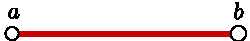
\includegraphics[width=3.5cm]{../Topicos/Figuras/aberto-a-aberto-b.pdf}
 \end{figure}
 \item Intervalo fechado: $[a, b]= \{x \in \R \mid a \leq x \leq b\}$;
 \begin{figure}[H]
 \centering
 
\includegraphics[width=3.5cm]{../Topicos/Figuras/fechado-a-fechado-b.pdf}
 \end{figure}
 \item Intervalo aberto à direita e fechado à esquerda: $[a, b[= \{x \in \R \mid a \leq x < b\}$;
 \begin{figure}[H]
 \centering
 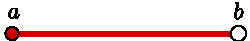
\includegraphics[width=3.5cm]{../Topicos/Figuras/fechado-a-aberto-b.pdf}
 \end{figure}
 \item Intervalo aberto à esquerda e fechado à direita: $]a, b]= \{x \in \R \mid a < x \leq b\}$.
 \begin{figure}[H]
 \centering
 
\includegraphics[width=3.5cm]{../Topicos/Figuras/aberto-a-fechado-b.pdf}
 \end{figure}
\end{itemize}



\textbf{Intervalos numéricos ilimitados}
\begin{itemize}
\item Conjunto dos números reais maiores que $a$: $[a, +\infty[ = \{ x \in \R \mid a < x \}$
 \begin{figure}[H]
 \centering
 
\includegraphics[width=3.5cm]{../Topicos/Figuras/aberto-a-inf.pdf}
 \end{figure}

\item Conjunto dos números reais maiores ou iguais à $a$: $[a, +\infty[ = \{ x \in \R \mid a \leq x \}$
 \begin{figure}[H]
 \centering
 
\includegraphics[width=3.5cm]{../Topicos/Figuras/fechado-a-inf.pdf}
 \end{figure}

\item Conjunto dos números reais menores que $b$: $]-\infty, b] = \{ x \in \R \mid x < b \}$
 \begin{figure}[H]
 \centering
 
\includegraphics[width=3.5cm]{../Topicos/Figuras/inf-aberto-b.pdf}
 \end{figure}

\item Conjunto dos números reais menores ou iguais à $b$: $]-\infty, b] = \{ x \in \R \mid x \leq b \}$
 \begin{figure}[H]
 \centering
 
\includegraphics[width=3.5cm]{../Topicos/Figuras/inf-fechado-b.pdf}
 \end{figure}

\item Conjunto dos números reais: $]-\infty, +\infty[ = \R$
 \begin{figure}[H]
 \centering
 
\includegraphics[width=7.5cm]{../Topicos/Figuras/reta.pdf}
 \end{figure}
\end{itemize}


\textbf{Outros subconjuntos dos números Reais}
\begin{itemize}
 \item Conjunto dos números reais não-nulos: $\R^{*}=\{x \in \R \mid x \neq 0\}$;
 \begin{figure}[H]
 \centering
 
\includegraphics[width=7.5cm]{../Topicos/Figuras/n-nulos.pdf}
 \end{figure}
 \item Conjunto dos números reais não-negativos: $\R_{+}=\{x \in \R \mid x \geq 0\}$;
 \begin{figure}[H]
 \centering
 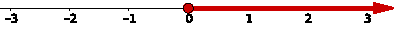
\includegraphics[width=7.5cm]{../Topicos/Figuras/n-negativos.pdf}
 \end{figure}
 \item Conjunto dos números reais positivos: $\R^{*}_{+}=\{x \in \R \mid x > 0\}$;
 \begin{figure}[H]
 \centering
 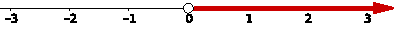
\includegraphics[width=7.5cm]{../Topicos/Figuras/positivos.pdf}
 \end{figure}
 \item Conjunto dos números reais não-positivos: $\R_{-}=\{x \in \R \mid x \leq 0\}$;
 \begin{figure}[H]
 \centering
 
\includegraphics[width=7.5cm]{../Topicos/Figuras/n-positivos.pdf}
 \end{figure}
 \item Conjunto dos números reais negativos: $\R^{*}_{-}=\{x \in \R \mid x < 0\}$.
 \begin{figure}[H]
 \centering
 
\includegraphics[width=7.5cm]{../Topicos/Figuras/negativos.pdf}
 \end{figure}
\end{itemize}
